%% METADATA
%% subject-code: DI01000051
%% subject-name: Fundamentals of Electronics
%% semester: 1
%% examination: Winter-2024
%% date: 07-01-2025
%% description: Solution guide for Fundamentals of Electronics
%% tags: study-material, solutions, gtu, DI01000051
%% END METADATA

\documentclass{article}

% content/resources/templates/preamble.tex
\usepackage[margin=0.6in]{geometry}
\author{Milav Dabgar}
\usepackage{amsmath,amssymb,amsthm}
\usepackage{booktabs}
\usepackage{multirow}
\usepackage{xcolor}
\usepackage{tcolorbox}
\tcbuselibrary{breakable,skins}
\usepackage[colorlinks=true,linkcolor=blue]{hyperref}
\usepackage{titlesec}
\usepackage{enumitem}
\usepackage{tikz}
\usepackage{pgfplots}
\usepackage{circuitikz}
\usepackage[version=4]{mhchem}
\usepackage{longtable}
\usepackage{array}
\usepackage{float}
\usepackage{caption}
\usepackage{listings}

\lstset{
  basicstyle=\small\ttfamily,
  breaklines=true,
  breakatwhitespace=false,
  postbreak=\mbox{\textcolor{red}{$\hookrightarrow$}\space},
  float=false,
  numbers=left,
  numberstyle=\tiny\color{gray},
  numbersep=10pt,
  xleftmargin=2em,
  keywordstyle=\color{blue},
  commentstyle=\color{green!60!black},
  stringstyle=\color{purple},
  backgroundcolor=\color{gray!5},
  showstringspaces=false,
  tabsize=2,
  captionpos=b,
  keepspaces=true,
  columns=flexible
}

\pgfplotsset{compat=1.18}
\usetikzlibrary{shapes,arrows,positioning,calc,patterns,decorations.pathmorphing,decorations.markings,arrows.meta}

% Color scheme
\definecolor{headcolor}{RGB}{0,102,204}
\definecolor{keycolor}{RGB}{220,20,60}
\definecolor{solutioncolor}{RGB}{34,139,34}
\definecolor{mnemoniccolor}{RGB}{148,0,211}
\definecolor{codecolor}{RGB}{0,0,100}

% Spacing
\setlength{\parskip}{3pt}
\setlist[itemize]{nosep}
\setlist[enumerate]{nosep}

% Title formatting
\titleformat{\section}{\Large\bfseries\color{headcolor}}{\thesection}{1em}{}
\titleformat{\subsection}{\large\bfseries\color{headcolor}}{\thesubsection}{1em}{}

% Pandoc tightlist compatibility
\providecommand{\tightlist}{%
  \setlength{\itemsep}{0pt}\setlength{\parskip}{0pt}}

% Pandoc longtable compatibility
\newcounter{none}
\def\thenone{}


\title{Fundamentals of Electronics (DI01000051) - Winter 2024 Solution}
\date{January 07, 2025}

\hypersetup{
  pdftitle={Fundamentals of Electronics (DI01000051) - Winter 2024 Solution},
  pdfsubject={GTU Exam Solution - Winter-2024},
  pdfauthor={Milav Dabgar},
  pdfkeywords={study-material, solutions, gtu, DI01000051},
  pdfcreator={xelatex}
}

\begin{document}
\maketitle

\setcounter{tocdepth}{5}
\tableofcontents
\newpage

% ========================================
% QUESTION 1(a): Active and Passive Components (3 marks)
% Demonstrates: Definitions, Examples, Comparison
% ========================================

\section{Question 1}
\subsection{Question 1(a) [3 marks]}
\textbf{Define Active and Passive Components with example.}

\subsubsection{Solution}
Electronic components are broadly classified into two categories: Active and Passive components based on their ability to generate or control energy.

\paragraph{Active Components:}
These are components that can generate energy (power) or control the flow of current. They require an external source of power to operate. They are capable of amplifying signals.
\begin{itemize}
    \item \textbf{Examples:} Transistors (BJT, FET), Diodes (Zener, Tunnel), Integrated Circuits (ICs), Batteries, Generators.
\end{itemize}

\paragraph{Passive Components:}
These are components that strictly receive energy, which they either dissipate (as heat), absorb, or store in an electric or magnetic field. They cannot generate power or amplify signals. They do not require an separate external power source to function (they work on the signal itself).
\begin{itemize}
    \item \textbf{Examples:} Resistors (dissipate energy), Capacitors (store electric energy), Inductors (store magnetic energy), Transformers.
\end{itemize}

\paragraph{Mnemonic:}
\emph{Active Adds Action (Gain/Control); Passive Plays Part (Stores/Dissipates).}

% ========================================
% QUESTION 1(b): LDR Construction and Working (4 marks)
% Demonstrates: Construction Diagram, Working Principle
% ========================================

\subsection{Question 1(b) [4 marks]}
\textbf{Explain construction and working of LDR.}

\subsubsection{Solution}
A Light Dependent Resistor (LDR), also known as a photoresistor, is a component whose resistance decreases as the intensity of incident light increases.

\paragraph{Construction:}
It consists of a light-sensitive material, typically Cadmium Sulphide (CdS), deposited on an insulating ceramic substrate.
\begin{enumerate}
    \item The semiconductor material is arranged in a zig-zag track to maximize the exposed surface area while keeping the device compact.
    \item Metal electrodes are placed at the ends of the zig-zag track to provide connections.
    \item The entire assembly is encapsulated in a transparent plastic or glass casing to protect it from moisture while allowing light to pass through.
\end{enumerate}

\paragraph{Diagram:}
\begin{figure}[H]
\centering
\begin{circuitikz}[scale=1.2]
    \draw (0,0) to[ldR, l=LDR, o-o] (3,0);
\end{circuitikz}
\caption{Symbol of LDR}
\end{figure}

\paragraph{Working:}
LDR works on the principle of \textbf{Photoconductivity}.
\begin{enumerate}
    \item \textbf{Dark Condition:} In the absence of light, the material has very few free electrons. It behaves almost like an insulator, offering very high resistance (Mega Ohms range).
    \item \textbf{Light Condition:} When light photons fall on the CdS material, they impart energy to the valence electrons.
    \item If the photon energy is sufficient, covalent bonds break, and electron-hole pairs are generated.
    \item These free charge carriers increase the conductivity of the material, thereby drastically reducing its resistance (drops to few hundred Ohms).
\end{enumerate}

\paragraph{Mnemonic:}
\emph{LDR: Light Drops Resistance (More Light = Less Resistance).}

% ========================================
% QUESTION 1(c): Capacitance & Electrolytic Capacitor (7 marks)
% Demonstrates: Definition, Diagrams, Detailed Working
% ========================================

\subsection{Question 1(c) [7 marks]}
\textbf{Define Capacitance and explain Aluminum Electrolytic wet type capacitor.}

\subsubsection{Solution}
\paragraph{Defintion of Capacitance:}
Capacitance (\(C\)) is the ability of a system to store an electric charge. It is defined as the ratio of the change in electric charge (\(Q\)) in a system to the corresponding change in its electric potential (\(V\)).
\[ C = \frac{Q}{V} \]
The unit of capacitance is Farad (F).

\paragraph{Aluminum Electrolytic Capacitor (Wet Type):}
This type of capacitor is used when large capacitance values are required (e.g., in power supply filters). It is a polarized component.

\paragraph{Construction:}
\begin{enumerate}
    \item \textbf{Anode:} A pure aluminum foil acts as the positive plate (anode). Its surface is etched to increase surface area. A thin layer of Aluminum Oxide (\(Al_2O_3\)) is formed on it, which acts as the \textbf{Dielectric}.
    \item \textbf{Cathode:} Another aluminum foil acts as the negative connection.
    \item \textbf{Electrolyte:} Between the plates, a paper separator soaked in a liquid electrolyte (e.g., borax or glycol) is placed. The electrolyte serves as the actual cathode, making contact with the oxide layer.
    \item The assembly is rolled into a cylindrical shape and housed in an aluminum can.
\end{enumerate}

\paragraph{Diagram:}
\begin{figure}[H]
\centering
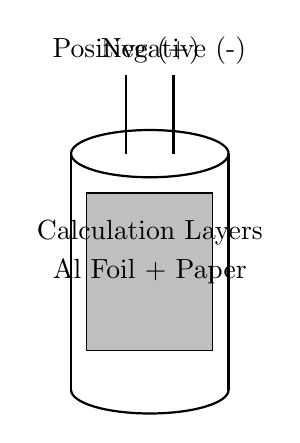
\begin{tikzpicture}
    % Cylinder body
    \draw[thick] (0,0) ellipse (1cm and 0.3cm);
    \draw[thick] (-1,0) -- (-1,-3);
    \draw[thick] (1,0) -- (1,-3);
    \draw[thick] (-1,-3) arc (180:360:1cm and 0.3cm);
    
    % Internal layers representation
    \draw[fill=lightgray] (-0.8,-0.5) rectangle (0.8,-2.5);
    \node at (0,-1) {Calculation Layers};
    \node at (0,-1.5) {Al Foil + Paper};
    
    % Leads
    \draw[thick] (-0.3,0) -- (-0.3,1) node[above] {Positive (+)};
    \draw[thick] (0.3,0) -- (0.3,1) node[above] {Negative (-)};
\end{tikzpicture}
\caption{Construction of Electrolytic Capacitor}
\end{figure}

\paragraph{Working:}
When a DC voltage is applied with correct polarity (Positive to Anode), the process of electrolysis maintains the thin oxide layer. This oxide layer is extremely thin, which allows for a very high capacitance value according to the formula \(C = \frac{\epsilon A}{d}\) (small \(d\)). If reverse polarity is applied, the oxide layer breaks down, causing a short circuit and potential explosion.

\paragraph{Mnemonic:}
\emph{Wet Paper Holds Charge; Polarity Matters (Oxide Dielectric).}

% ========================================
% QUESTION 1(c) OR: Resistor Color Code (7 marks)
% Demonstrates: Table, Calculation, Example
% ========================================

\subsection{Question 1(c) OR [7 marks]}
\textbf{Explain the color band coding method of Resistor. Write color band of 32 \(\Omega\) \(\pm\)10\% resistance.}

\subsubsection{Solution}
Resistor color coding is an international standard used to indicate the resistance value and tolerance of small resistors. Since resistors are often too small to have numbers printed on them legibly, colored bands are painted on the body to represent their values.

\paragraph{Color Code Table:}
The Electronic Industries Alliance (EIA) defines the color code system. Each color corresponds to a specific digit (0-9), a multiplier factor, and a tolerance percentage.
\begin{table}[H]
\centering
\caption{Resistor Color Codes}
\begin{tabularx}{\textwidth}{|l|X|X|X|}
\hline
\textbf{Color} & \textbf{Digit} & \textbf{Multiplier} & \textbf{Tolerance} \\
\hline
Black & 0 & \(10^0\) & - \\
Brown & 1 & \(10^1\) & \(\pm 1\%\) \\
Red & 2 & \(10^2\) & \(\pm 2\%\) \\
Orange & 3 & \(10^3\) & - \\
Yellow & 4 & \(10^4\) & - \\
Green & 5 & \(10^5\) & \(\pm 0.5\%\) \\
Blue & 6 & \(10^6\) & \(\pm 0.25\%\) \\
Violet & 7 & \(10^7\) & \(\pm 0.1\%\) \\
Grey & 8 & \(10^8\) & - \\
White & 9 & \(10^9\) & - \\
Gold & - & \(10^{-1}\) & \(\pm 5\%\) \\
Silver & - & \(10^{-2}\) & \(\pm 10\%\) \\
\hline
\end{tabularx}
\end{table}

\paragraph{4-Band System Explanation:}
The most common resistor types use a 4-band code. Reading from left to right:
\begin{itemize}
    \item \textbf{1st Band (First Significant Digit):} This band represents the first digit of the resistance value.
    \item \textbf{2nd Band (Second Significant Digit):} This band represents the second digit of the resistance value.
    \item \textbf{3rd Band (Multiplier):} This band indicates the number of zeros to add after the first two digits, or effectively the power of 10 by which the significant digits are multiplied.
    \item \textbf{4th Band (Tolerance):} This band usually follows a gap and indicates the precision of the resistor. Silver indicates \(\pm 10\%\) and Gold indicates \(\pm 5\%\).
\end{itemize}

\paragraph{Calculation for 32 \(\Omega\) \(\pm\)10\%:}
\subparagraph{Value Breakdown:}
We are given a resistance value of \(32 \Omega\) with a tolerance of \(10\%\). We break this down into the standard format:
\[ Value = (1st Digit)(2nd Digit) \times Multiplier \]
\[ 32 \Omega = 32 \times 1 \]
\[ 32 \Omega = 32 \times 10^0 \]

\subparagraph{Mapping to Colors:}
Now, we map these components to their respective colors:
\begin{enumerate}
    \item \textbf{1st Band (Digit 3):} Looking at the table, the digit 3 corresponds to the color \textbf{Orange}.
    \item \textbf{2nd Band (Digit 2):} The digit 2 corresponds to the color \textbf{Red}.
    \item \textbf{3rd Band (Multiplier \(10^0\)):} The multiplier is \(1\) (since we need exactly 32, not 320 or 3200). The table shows that \(10^0\) corresponds to the color \textbf{Black}.
    \item \textbf{4th Band (Tolerance \(\pm 10\%\)):} The tolerance is specified as \(10\%\), which corresponds to the color \textbf{Silver}.
\end{enumerate}

\textbf{Final Answer:} The sequence of color bands on the resistor body would be \textbf{Orange - Red - Black - Silver}.

\paragraph{Mnemonic:}
\emph{B B R O Y of Great Britain had a Very Good Wife (GS). Black-0, Brown-1, Red-2\dots}

% ========================================
% QUESTION 2(a): Definitions (3 marks)
% Demonstrates: Precise definitions
% ========================================

\section{Question 2}
\subsection{Question 2(a) [3 marks]}
\textbf{Define following terms: 1) Rectifier 2) Ripple factor 3) Filter}

\subsubsection{Solution}
\begin{enumerate}
    \item \textbf{Rectifier:} A rectifier is an electronic device or circuit that converts Alternating Current (AC) into Direct Current (DC). It typically uses one or more diodes to allow current to flow in only one direction.
    \item \textbf{Ripple Factor:} The output of a rectifier is not pure DC but contains some AC components called ripples. Ripple factor is defined as the ratio of the RMS value of the AC component of the output voltage to the DC component of the output voltage.
    \[ \text{Ripple Factor} (\gamma) = \frac{V_{ac(rms)}}{V_{dc}} \]
    \item \textbf{Filter:} A filter is a circuit used after the rectifier to remove the unwanted AC components (ripples) from the pulsating DC output and provide a steady/smooth DC voltage to the load. It usually consists of capacitors and inductors.
\end{enumerate}

\paragraph{Mnemonic:}
\emph{RRF: Rectify converts, Ripple measures AC junk, Filter cleans it up.}


% ========================================
% QUESTION 2(b): Positive Clipper (4 marks)
% Demonstrates: Circuit Diagram, Waveforms, Working
% ========================================

\subsection{Question 2(b) [4 marks]}
\textbf{Draw and explain positive clipper circuit with waveform.}

\subsubsection{Solution}
A positive clipper is a circuit that removes the positive half cycle of the input AC signal.

\paragraph{Circuit Diagram:}
The diode is connected in parallel with the load (shunt clipper) or series. Here is a Series Positive Clipper.
\begin{figure}[H]
\centering
\begin{circuitikz}[scale=1]
    \draw (0,0) to[sV, l=Input] (0,2);
    \draw (0,2) to[diode, l=D, -*] (3,2);
    \draw (3,2) to[R, l=\(R_L\), -*] (3,0);
    \draw (3,0) -- (0,0);
    \draw (3,2) -- (4,2) node[right] {Output};
    \draw (3,0) -- (4,0);
\end{circuitikz}
\caption{Series Positive Clipper}
\end{figure}

\paragraph{Working:}
\begin{enumerate}
    \item \textbf{Positive Half Cycle:} During the positive half cycle of the input, the diode is reverse biased (Cathode positive with respect to Anode). It acts as an open switch. No current flows through the load resistor \(R_L\). Hence, output voltage \(V_o = 0\).
    \item \textbf{Negative Half Cycle:} During the negative half cycle, the diode is forward biased (Anode positive with respect to Cathode). It acts as a closed switch. Current flows through the load, and the output follows the negative input cycle.
\end{enumerate}

\paragraph{Waveforms:}
The input shows a full sine wave, while the output shows only the negative half cycles.

\paragraph{Mnemonic:}
\emph{Positive Clipper: Diode Blocks Plus (Reverse Biased in Positive).}


% ========================================
% QUESTION 2(c): Full Wave Rectifier (Center Tap) (7 marks)
% Demonstrates: Circuit, Operation, Waveforms
% ========================================

\subsection{Question 2(c) [7 marks]}
\textbf{Explain working of full wave rectifier with two diodes.}

\subsubsection{Solution}
A Full Wave Rectifier converts both halves of the AC cycle into pulsating DC. The center-tapped full wave rectifier uses two diodes and a center-tapped transformer.

\paragraph{Circuit Diagram:}
\begin{figure}[H]
\centering
\begin{circuitikz}[scale=1]
    \draw (0,0) node[transformer core] (T) {};
    \draw (T.A1) -- ++(-1,0) to[sV, l=AC Input] ++(0,-2) -- (T.A2);
    \draw (T.B1) to[diode, l=D1] ++(2,0) coordinate (top);
    \draw (T.B2) to[diode, l=D2] ++(2,0) coordinate (bot);
    \draw (top) -- (bot) coordinate[midway] (mid);
    \draw (T.base) -- ++(1,0) coordinate (center); 
    \draw (mid) to[R, l=\(R_L\)] (center);
\end{circuitikz}
\caption{Center Tapped Full Wave Rectifier}
\end{figure}

\paragraph{Construction:}
It consists of a center-tapped transformer with secondary winding split into two halves. Two diodes \(D_1\) and \(D_2\) are connected to the ends of the secondary winding. The load resistor \(R_L\) is connected between the common cathode point of diodes and the center tap.

\paragraph{Working Explanation:}
\subparagraph{Positive Half Cycle:}
When point A (top) is positive with respect to center tap C, and point B (bottom) is negative:
\begin{itemize}
    \item Diode \(D_1\) is forward biased and conducts.
    \item Diode \(D_2\) is reverse biased and stays OFF.
    \item Current flows through \(D_1\), load \(R_L\), and back to the center tap.
\end{itemize}

\subparagraph{Negative Half Cycle:}
When point A is negative and point B is positive with respect to center tap C:
\begin{itemize}
    \item Diode \(D_2\) is forward biased and conducts.
    \item Diode \(D_1\) is reverse biased and stays OFF.
    \item Current flows through \(D_2\), load \(R_L\), and back to the center tap.
\end{itemize}
In both cases, current flows through the load \(R_L\) in the \textbf{same direction}, providing a unidirectional output.

\paragraph{Mnemonic:}
\emph{Center Tap: Two Diodes take turns; One pushes, One waits.}


% ========================================
% QUESTION 2(a) OR: Rectifier Applications (3 marks)
% Demonstrates: List of uses
% ========================================

\subsection{Question 2(a) OR [3 marks]}
\textbf{Define rectifier and write its applications.}

\subsubsection{Solution}
\paragraph{Definition:}
A rectifier is a device that converts alternating current (AC) to direct current (DC).

\paragraph{Applications:}
Rectifiers are essential components in electronics and are used in:
\begin{enumerate}
    \item \textbf{DC Power Supplies:} To provide DC voltage for electronic circuits (computers, TVs, mobile chargers).
    \item \textbf{Battery Charging:} To charge batteries in vehicles, UPS systems, and portable devices.
    \item \textbf{Demodulation:} In radio receivers to extract the signal (AM detection).
    \item \textbf{Electroplating:} To provide steady DC current for industrial chemical processes.
\end{enumerate}

\paragraph{Mnemonic:}
\emph{Rectifier: AC to DC. Used in Power, Charge, Radio, Plating.}


% ========================================
% QUESTION 2(b) OR: Pi Filter (4 marks)
% Demonstrates: Circuit, Operation
% ========================================

\subsection{Question 2(b) OR [4 marks]}
\textbf{Explain working of Pi(\(\pi\)) type capacitor filter.}

\subsubsection{Solution}
A Pi filter (also called CLC filter) consists of two capacitors and one inductor arranged in the shape of the Greek letter Pi (\(\pi\)).

\paragraph{Circuit Diagram:}
\begin{figure}[H]
\centering
\begin{circuitikz}[scale=1]
    \draw (0,1) to[short, o-] (1,1) to[C, l=C1] (1,0) to[short, -o] (0,0);
    \draw (1,1) to[L, l=L] (3,1) to[C, l=C2] (3,0) -- (1,0); 
    \draw (3,1) -- (4,1) to[R, l=Load] (4,0) -- (3,0);
\end{circuitikz}
\caption{Pi Filter Circuit}
\end{figure}

\paragraph{Working:}
\begin{enumerate}
    \item \textbf{Capacitor \(C_1\):} This first capacitor is connected across the rectifier output. It offers low reactance to AC ripples and bypasses most of them to the ground. It charges to the peak voltage.
    \item \textbf{Inductor \(L\):} The series inductor offers high reactance to any remaining AC components, blocking them, while offering almost zero resistance to DC current.
    \item \textbf{Capacitor \(C_2\):} The second capacitor further bypasses any residual AC ripples that passed through the inductor, ensuring a very smooth DC output across the load.
\end{enumerate}

\paragraph{Mnemonic:}
\emph{Pi Filter: C-L-C Sandwich. Bypasses AC, Blocks AC, Smooths DC.}


% ========================================
% QUESTION 2(c) OR: Half Wave vs Full Wave Bridge (7 marks)
% Demonstrates: Comparison Table
% ========================================

\subsection{Question 2(c) OR [7 marks]}
\textbf{Compare half wave and full wave bridge rectifier.}

\subsubsection{Solution}
Comparison between Half Wave and Full Wave Bridge Rectifier:

\begin{table}[H]
\centering
\caption{Comparison of Rectifiers}
\begin{tabularx}{\textwidth}{|X|X|X|}
\hline
\textbf{Parameter} & \textbf{Half Wave Rectifier} & \textbf{Bridge Rectifier} \\
\hline
Number of Diodes & Uses 1 Diode. & Uses 4 Diodes. \\
\hline
Transformer & Simple transformer required. & Simple transformer required (No center tap needed). \\
\hline
Efficiency & Low efficiency (Max 40.6\%). & High efficiency (Max 81.2\%). \\
\hline
Ripple Factor & High Ripple (1.21). Output is pulsating. & Low Ripple (0.48). Output is smoother. \\
\hline
Peak Inverse Voltage (PIV) & PIV rating is \(V_m\). & PIV rating is \(V_m\). \\
\hline
Output Frequency & Equal to input frequency (\(f_{in}\)). & Double input frequency (\(2f_{in}\)). \\
\hline
Cost & Very low cost. & Moderate (cost of 4 diodes). \\
\hline
\end{tabularx}
\end{table}

\subparagraph{Detailed Comparison Points:}
\begin{itemize}
    \item \textbf{Ripple Factor:} The half-wave rectifier has a very high ripple factor (\(\gamma = 1.21\)), which means the AC component in the output is larger than the DC component. This requires heavy and expensive filtering circuits to smooth out. In contrast, the bridge rectifier has a much lower ripple factor (\(\gamma = 0.48\)), producing a smoother output that is easier to filter.
    \item \textbf{Transformer Utilization:} In a half-wave rectifier, current flows in the transformer secondary winding only during one half-cycle. This causes DC saturation of the core and results in poor Transformer Utilization Factor (TUF). The bridge rectifier utilizes both half-cycles effectively, has no net DC current in the transformer, and thus offers a much higher TUF.
    \item \textbf{Output Power:} For the same AC input voltage, a bridge rectifier provides significantly higher DC output power compared to a half-wave rectifier because it utilizes the full AC wave.
\end{itemize}

\subparagraph{Summary:}
The Bridge rectifier is generally essential for high-quality DC power supplies due to its higher efficiency and lower ripple, despite using more diodes. Half wave rectifiers are rarely used except for very low-power, non-critical applications.

\paragraph{Mnemonic:}
\emph{Bridge is Better: Double Efficiency, Half Ripple, Needs 4 Diodes.}

% ========================================
% QUESTION 3(a): Symbols (3 marks)
% Demonstrates: Circuit Symbols
% ========================================

\section{Question 3}
\subsection{Question 3(a) [3 marks]}
\textbf{Draw symbols of: 1) Zener Diode 2) LED 3) Varactor Diode.}

\subsubsection{Solution}
\begin{figure}[H]
\centering
\begin{tabularx}{\textwidth}{X X X}
    \centering
    \begin{circuitikz}[scale=1]
        \draw (0,0) to[zD] (2,0);
        \node at (1,-0.5) {Zener Diode};
    \end{circuitikz} &
    \centering
    \begin{circuitikz}[scale=1]
        \draw (0,0) to[leD] (2,0);
        \node at (1,-0.5) {LED};
    \end{circuitikz} &
    \centering
    \begin{circuitikz}[scale=1]
        \draw (0,0) to[D] (2,0); % vD not supported, using D
        \node at (1,-0.5) {Varactor Diode};
    \end{circuitikz}
\end{tabularx}
\caption{Symbols of Special Diodes}
\end{figure}

\begin{enumerate}
    \item \textbf{Zener Diode:} It works in reverse breakdown region. Symbol has a `Z' shape cathode.
    \item \textbf{LED (Light Emitting Diode):} Detailed explanation not required, but it emits light. Arrows point outward.
    \item \textbf{Varactor Diode:} Acts as a variable capacitor. Symbol includes a capacitor plate.
\end{enumerate}

\paragraph{Mnemonic:}
\emph{Zener bends like Z, LED shines out, Varactor is a Variable Cap.}


% ========================================
% QUESTION 3(b): Zener Voltage Regulator (4 marks)
% Demonstrates: Circuit, Operation
% ========================================

\subsection{Question 3(b) [4 marks]}
\textbf{Explain working of Zener diode as voltage regulator.}

\subsubsection{Solution}
A Zener diode voltage regulator maintains a constant output voltage despite changes in input voltage or load current.

\paragraph{Circuit Diagram:}
\begin{figure}[H]
\centering
\begin{circuitikz}[scale=1]
    \draw (0,0) to[sV, l=\(V_{in}\)] (0,3) to[R, l=\(R_S\)] (3,3) coordinate (top);
    \draw (top) to[zD, l=\(D_Z\), *-*] (3,0); 
    \draw (top) -- (5,3) to[R, l=\(R_L\)] (5,0) -- (0,0);
    \draw (5,3) -- (6,3) node[right] {+ \(V_{out}\)};
    \draw (5,0) -- (6,0) node[right] {-};
\end{circuitikz}
\caption{Zener Voltage Regulator}
\end{figure}

\paragraph{Working Principle:}
The Zener diode is connected in reverse bias parallel to the load \(R_L\). The series resistor \(R_S\) limits the current.
\begin{enumerate}
    \item \textbf{Regulation against Input Variation:} If input voltage \(V_{in}\) increases, the total current increases. The Zener diode conducts more current (\(I_Z\) increases), causing a larger voltage drop across \(R_S\). The voltage across the Zener (and parallel Load) remains constant at \(V_Z\).
    \item \textbf{Regulation against Load Variation:} If load current \(I_L\) changes (e.g., decreases), the Zener current \(I_Z\) increases by the same amount to keep total current constant (approximately). Thus, voltage \(V_{out}\) remains clamped at \(V_Z\).
\end{enumerate}

\paragraph{Mnemonic:}
\emph{Zener acts like a Wall at \(V_Z\). Excess flows through Zener, Load stays safe.}


% ========================================
% QUESTION 3(c): NPN Transistor Working (7 marks)
% Demonstrates: Structure, Biasing, Electron flow
% ========================================

\subsection{Question 3(c) [7 marks]}
\textbf{Explain working of NPN transistor.}

\subsubsection{Solution}
An NPN transistor consists of a P-type semiconductor layer sandwiched between two N-type layers.

\paragraph{Construction \& Biasing:}
\begin{itemize}
    \item \textbf{Emitter (N):} Heavily doped, supplies electrons.
    \item \textbf{Base (P):} Lightly doped and very thin, controls flow.
    \item \textbf{Collector (N):} Moderately doped, collects electrons.
\end{itemize}
For active region operation, the Emitter-Base junction is Forward Biased, and Collector-Base junction is Reverse Biased.

\paragraph{Working Diagram:}
\begin{figure}[H]
\centering
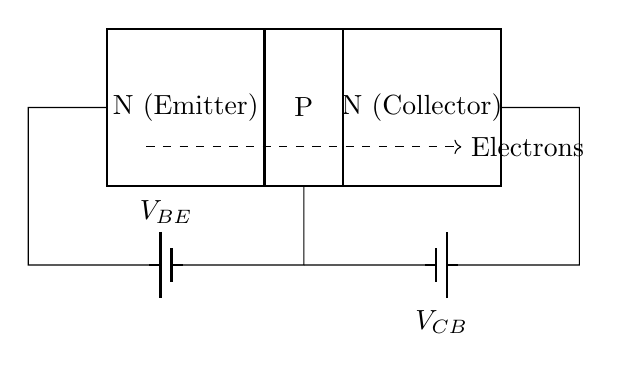
\begin{tikzpicture}[scale=1]
    % NPN Block
    \draw[thick] (0,0) rectangle (2,2) node[midway] {N (Emitter)};
    \draw[thick] (2,0) rectangle (3,2) node[midway] {P};
    \draw[thick] (3,0) rectangle (5,2) node[midway] {N (Collector)};
    
    % Biasing
    \draw (0,1) -- (-1,1) -- (-1,-1) to[battery1, l=\(V_{BE}\)] (2.5,-1) -- (2.5,0);
    \draw (5,1) -- (6,1) -- (6,-1) to[battery1, l=\(V_{CB}\)] (2.5,-1);
    
    % Electron Flow
    \draw[->, dashed] (0.5, 0.5) -- (4.5, 0.5) node[right] {Electrons};
\end{tikzpicture}
\caption{NPN Transistor Biasing and Flow}
\end{figure}

\paragraph{Operation:}
\subparagraph{Electron Injection:}
Since the Emitter-Base junction is forward biased, electrons from the N-type emitter are pushed towards the base.
\subparagraph{Base Transport:}
The base is very thin and lightly doped. Only a few electrons (about 5\%) recombine with holes in the P-region to form Base Current (\(I_B\)).
\subparagraph{Collection:}
The remaining 95\% of electrons cross the base and reach the collector junction. Since the Collector-Base junction is reverse biased (Positive connected to Collector), these electrons are strongly attracted by the positive potential of the collector and flow out to form Collector Current (\(I_C\)).

\subparagraph{Current Equation:}
Applying Kirchhoff's Current Law (KCL):
\[ I_E = I_B + I_C \]
Where \(I_E\) is Emitter Current, \(I_B\) is Base Current, and \(I_C\) is Collector Current. Since \(I_B\) is very small, \(I_C \approx I_E\).

\paragraph{Mnemonic:}
\emph{NPN: Not Pointing In (Arrow points out). Emitter Emits, Base Controls, Collector Collects.}


% ========================================
% QUESTION 3(a) OR: Transistor Definition (3 marks)
% Demonstrates: Definition
% ========================================

\subsection{Question 3(a) OR [3 marks]}
\textbf{Define Transistor and list its types.}

\subsubsection{Solution}
\paragraph{Definition:}
A Transistor is a three-terminal semiconductor device used to amplify or switch electrical signals and power. It is composed of semiconductor material usually with at least three terminals for connection to an external circuit.

\paragraph{Types of Transistors:}
Transistors are broadly classified into two main families, each with specific operating principles:
\begin{enumerate}
    \item \textbf{BJT (Bipolar Junction Transistor):} Controlled by current. It uses both electrons and holes for conduction.
    \begin{itemize}
        \item NPN Transistor: Electrons are majority carriers (faster, popular).
        \item PNP Transistor: Holes are majority carriers.
    \end{itemize}
    \item \textbf{FET (Field Effect Transistor):} Controlled by voltage. It uses only one type of charge carrier (Unipolar).
    \begin{itemize}
        \item JFET (Junction FET): Simple construction, high input impedance. (N-channel, P-channel).
        \item MOSFET (Metal Oxide Semiconductor FET): Very high input impedance, used in digital circuits. (Depletion Type, Enhancement Type).
    \end{itemize}
\end{enumerate}

\paragraph{Applications:}
Transistors are the building blocks of modern electronics, used in amplifiers, switches, voltage regulators, and oscillators.

\paragraph{Mnemonic:}
\emph{Transistor = Transfer + Resistor. BJT (Bi) and FET (Field) are main families.}


% ========================================
% QUESTION 3(b) OR: PNP Transistor Construction (4 marks)
% Demonstrates: Block diagram
% ========================================

\subsection{Question 3(b) OR [4 marks]}
\textbf{Draw and explain construct of PNP transistor.}

\subsubsection{Solution}
A PNP transistor is formed by sandwiching a thin layer of N-type semiconductor between two layers of P-type semiconductor.

\paragraph{Structure Diagram:}
\begin{figure}[H]
\centering
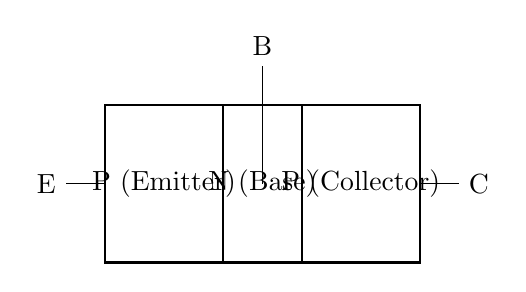
\begin{tikzpicture}[scale=1]
    \draw[thick] (0,0) rectangle (1.5,2) node[midway] {P (Emitter)};
    \draw[thick] (1.5,0) rectangle (2.5,2) node[midway] {N (Base)};
    \draw[thick] (2.5,0) rectangle (4,2) node[midway] {P (Collector)};
    \draw (0,1) -- (-0.5,1) node[left] {E};
    \draw (2,1) -- (2,2.5) node[above] {B};
    \draw (4,1) -- (4.5,1) node[right] {C};
\end{tikzpicture}
\caption{PNP Transistor Construction}
\end{figure}

\paragraph{Terminals:}
\begin{enumerate}
    \item \textbf{Emitter (E):} P-type region. It is heavily doped to supply majority charge carriers (Holes).
    \item \textbf{Base (B):} N-type region. It is very thin and lightly doped. It controls the flow of holes from Emitter to Collector.
    \item \textbf{Collector (C):} P-type region. It is moderately doped and larger in size than emitter to dissipate heat. It collects the holes supplied by the emitter.
\end{enumerate}

\paragraph{Mnemonic:}
\emph{PNP: Pointing In (Arrow points in). P-N-P Sandwich.}


% ========================================
% QUESTION 3(c) OR: PN Junction Diode V-I Characteristics (7 marks)
% Demonstrates: Graph, Explanation
% ========================================

\subsection{Question 3(c) OR [7 marks]}
\textbf{Explain V-I characteristics of PN junction diode.}

\subsubsection{Solution}
The V-I characteristic curve shows the relationship between the voltage across the diode (\(V\)) and the current flowing through it (\(I\)).

\paragraph{Characteristics Graph:}
\begin{figure}[H]
\centering
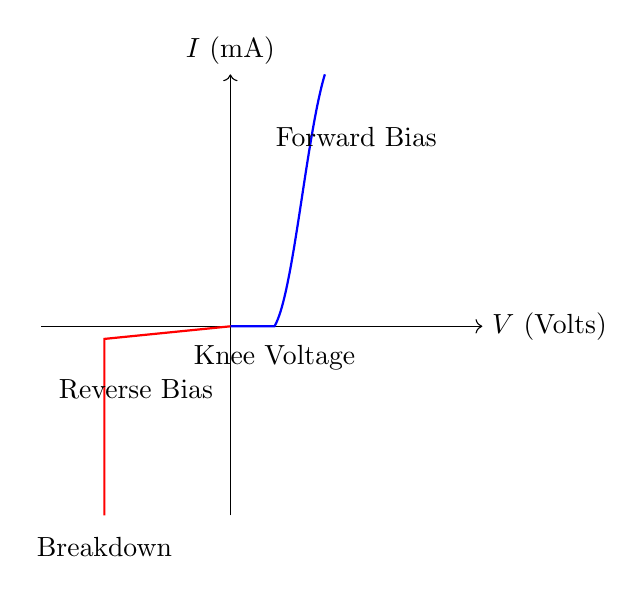
\begin{tikzpicture}[scale=0.8]
    \draw[->] (-3,0) -- (4,0) node[right] {\(V\) (Volts)};
    \draw[->] (0,-3) -- (0,4) node[above] {\(I\) (mA)};
    
    % Forward Bias curve
    \draw[thick, blue] (0,0) -- (0.7,0) .. controls (1,0.5) and (1.2,3) .. (1.5,4);
    \node at (2,3) {Forward Bias};
    \node at (0.7,-0.5) {Knee Voltage};

    % Reverse Bias curve
    \draw[thick, red] (0,0) -- (-2, -0.2) -- (-2, -3);
    \node at (-1.5,-1) {Reverse Bias};
    \node at (-2,-3.5) {Breakdown};
\end{tikzpicture}
\caption{V-I Characteristics of PN Diode}
\end{figure}

\paragraph{Explanation:}
\subparagraph{Forward Bias Region:}
\begin{itemize}
    \item When the diode is forward biased (Anode positive), initially negligible current flows until the barrier potential is overcome.
    \item \textbf{Knee Voltage (Cut-in Voltage):} This is the voltage at which current starts increasing rapidly. For Silicon, it is approx \(0.7V\), and for Germanium, approx \(0.3V\).
    \item Beyond this voltage, current increases exponentially with voltage.
\end{itemize}

\subparagraph{Reverse Bias Region:}
\begin{itemize}
    \item When reverse biased (Anode negative), a very small current called \textbf{Reverse Saturation Current} (\(I_0\)) flows due to minority carriers. This current is temperature dependent but almost independent of voltage up to breakdown.
    \item The depletion region width increases in reverse bias, preventing majority carrier flow.
    \item \textbf{Reverse Breakdown:} If reverse voltage is increased beyond a limit (Breakdown Voltage), the covalent bonds break (Zener or Avalanche effect), and a large current flows, potentially damaging the diode if not limited.
\end{itemize}

\paragraph{Applications based on Characteristics:}
\begin{itemize}
    \item \textbf{Rectifiers:} Uses the forward bias property to convert AC to DC.
    \item \textbf{Switches:} Acts as a closed switch in forward bias and open switch in reverse bias.
    \item \textbf{Protection Circuits:} Prevents reverse polarity damage.
\end{itemize}

\paragraph{Mnemonic:}
\emph{Forward: Obstacle at 0.7V then FREE FLOW. Reverse: Wall holds until it BREAKS.}

% ========================================
% QUESTION 4(a): PNP/NPN Symbols & Construction (3 marks)
% Demonstrates: Symbols, Block Diagram
% ========================================

\section{Question 4}
\subsection{Question 4(a) [3 marks]}
\textbf{Draw symbols and construction of PNP and NPN transistor.}

\subsubsection{Solution}
\paragraph{Symbols:}
\begin{figure}[H]
\centering
\begin{tabularx}{\textwidth}{X X}
    \centering
    \begin{circuitikz}[scale=1]
        \draw (0,0) node[npn] (T) {};
        \node at (T) [right=0.5cm] {NPN (Not Pointing In)};
    \end{circuitikz} &
    \centering
    \begin{circuitikz}[scale=1]
        \draw (0,0) node[pnp] (T) {};
        \node at (T) [right=0.5cm] {PNP (Pointing In)};
    \end{circuitikz}
\end{tabularx}
\caption{Transistor Symbols}
\end{figure}

\paragraph{Construction Block Diagrams:}
\begin{figure}[H]
\centering
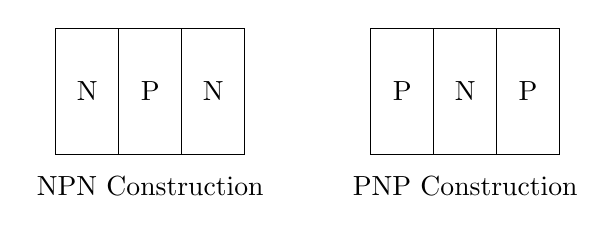
\begin{tikzpicture}[scale=0.8]
    % NPN
    \draw (0,0) rectangle (1,2) node[midway] {N};
    \draw (1,0) rectangle (2,2) node[midway] {P};
    \draw (2,0) rectangle (3,2) node[midway] {N};
    \node at (1.5,-0.5) {NPN Construction};
    
    % PNP
    \draw (5,0) rectangle (6,2) node[midway] {P};
    \draw (6,0) rectangle (7,2) node[midway] {N};
    \draw (7,0) rectangle (8,2) node[midway] {P};
    \node at (6.5,-0.5) {PNP Construction};
\end{tikzpicture}
\caption{Construction Structure}
\end{figure}

\paragraph{Mnemonic:}
\emph{NPN: Arrow OUT. PNP: Arrow IN.}


% ========================================
% QUESTION 4(b): CE Characteristics (4 marks)
% Demonstrates: Graph
% ========================================

\subsection{Question 4(b) [4 marks]}
\textbf{Draw and explain input and output characteristics of CE configuration.}

\subsubsection{Solution}
Common Emitter (CE) configuration is the most widely used configuration due to high current and voltage gain.

\paragraph{Input Characteristics:}
It is the graph of Input Current (\(I_B\)) vs Input Voltage (\(V_{BE}\)) at constant Output Voltage (\(V_{CE}\)).
\begin{itemize}
    \item It resembles a forward-biased diode characteristic.
    \item As \(V_{BE}\) increases beyond cut-in voltage (0.7V for Si), \(I_B\) increases rapidly.
    \item Higher \(V_{CE}\) shifts the curve slightly to the right due to the Early Effect.
\end{itemize}

\paragraph{Output Characteristics:}
It is the graph of Output Current (\(I_C\)) vs Output Voltage (\(V_{CE}\)) at constant Input Current (\(I_B\)).
\begin{itemize}
    \item \textbf{Active Region:} \(I_C\) is almost constant and proportional to \(I_B\). Normal amplifier operation.
    \item \textbf{Saturation Region:} Both junctions are forward biased. \(V_{CE}\) is very low.
    \item \textbf{Cut-off Region:} Both junctions are reverse biased. \(I_C \approx 0\).
\end{itemize}

\paragraph{Mnemonic:}
\emph{Input like Diode. Output like Steps (Flat lines controlled by \(I_B\)).}


% ========================================
% QUESTION 4(c): Current Gain Relation (7 marks)
% Demonstrates: Derivation
% ========================================

\subsection{Question 4(c) [7 marks]}
\textbf{Derive relation between \(\alpha\) and \(\beta\).}

\subsubsection{Solution}
\paragraph{Definitions:}
\begin{itemize}
    \item \(\alpha\) (Alpha): Current gain in Common Base (CB) configuration.
    \[ \alpha = \frac{I_C}{I_E} \]
    \item \(\beta\) (Beta): Current gain in Common Emitter (CE) configuration.
    \[ \beta = \frac{I_C}{I_B} \]
\end{itemize}

\paragraph{Derivation Steps:}
We begin with the fundamental transistor current relationship, which states that the Emitter current is the sum of Base current and Collector current:
\[ I_E = I_B + I_C \]
Our goal is to express \(\alpha\) (CB gain) in terms of \(\beta\) (CE gain).
Step 1: Divide the entire equation by the Collector current \(I_C\):
\[ \frac{I_E}{I_C} = \frac{I_B}{I_C} + \frac{I_C}{I_C} \]
Step 2: Substitute the definitions \(\frac{I_E}{I_C} = \frac{1}{\alpha}\) and \(\frac{I_B}{I_C} = \frac{1}{\beta}\) into the equation:
\[ \frac{1}{\alpha} = \frac{1}{\beta} + 1 \]
Step 3: Solve for \(\alpha\). Take the Least Common Multiple (LCM) on the right side:
\[ \frac{1}{\alpha} = \frac{1 + \beta}{\beta} \]
Step 4: Invert both sides to isolate \(\alpha\):
\[ \alpha = \frac{\beta}{1 + \beta} \]

Conversely, to find \(\beta\) in terms of \(\alpha\), we rearrange the inverse equation:
\[ \frac{1}{\beta} = \frac{1}{\alpha} - 1 = \frac{1 - \alpha}{\alpha} \]
Inverting gives:
\[ \beta = \frac{\alpha}{1 - \alpha} \]
This shows that \(\beta\) is much larger than \(\alpha\) because the denominator \((1-\alpha)\) is very small (since \(\alpha \approx 0.99\)).
For example, if \(\alpha = 0.99\), then \(\beta = \frac{0.99}{0.01} = 99\).

\paragraph{Relationship with Gamma (\(\gamma\)):}
\(\gamma\) is the current gain of Common Collector (CC) configuration, defined as \(\gamma = I_E / I_B\).
From the relation \(I_E = I_B + I_C\), dividing by \(I_B\):
\[ \frac{I_E}{I_B} = 1 + \frac{I_C}{I_B} \]
\[ \gamma = 1 + \beta \]
Since \(\beta\) is typically large (50-300), \(\gamma\) is approximately equal to \(\beta\). This confirms that CC configuration also has very high current gain, making it useful as a voltage buffer.

\paragraph{Mnemonic:}
\emph{\(\beta\) is Big (Greater than 1). \(\alpha\) is Always less than 1.}


% ========================================
% QUESTION 4(a) OR: Transistor Regions (3 marks)
% Demonstrates: List
% ========================================

\subsection{Question 4(a) OR [3 marks]}
\textbf{List operating regions of transistor.}

\subsubsection{Solution}
A transistor has three main operating regions based on the biasing of its two junctions (Emitter-Base and Collector-Base).

\begin{enumerate}
    \item \textbf{Active Region:}
    \begin{itemize}
        \item \textbf{Biasing:} Emitter-Base junction is Forward Biased, while Collector-Base junction is Reverse Biased.
        \item \textbf{Current:} Output current \(I_C\) is controlled by Input current \(I_B\) (\(I_C = \beta I_B\)).
        \item \textbf{Application:} Used for amplification of signals (Linear Amplifier).
    \end{itemize}
    \item \textbf{Saturation Region:}
    \begin{itemize}
        \item \textbf{Biasing:} Both Emitter-Base and Collector-Base junctions are Forward Biased.
        \item \textbf{Current:} Maximum Collector current flows independently of base current. \(V_{CE}\) is nearly zero (0.2V).
        \item \textbf{Application:} Acts as a Closed Switch (ON state) in digital logic.
    \end{itemize}
    \item \textbf{Cut-off Region:}
    \begin{itemize}
        \item \textbf{Biasing:} Both Emitter-Base and Collector-Base junctions are Reverse Biased.
        \item \textbf{Current:} Ideally zero collector current flows (minor leakage current only).
        \item \textbf{Application:} Acts as an Open Switch (OFF state).
    \end{itemize}
\end{enumerate}

\paragraph{Mnemonic:}
\emph{Active (FR) = Amplifier. Saturation (FF) = Switch ON. Cut-off (RR) = Switch OFF.}


% ========================================
% QUESTION 4(b) OR: Transistor as Amplifier (4 marks)
% Demonstrates: Circuit
% ========================================

\subsection{Question 4(b) OR [4 marks]}
\textbf{Explain transistor as an amplifier.}

\subsubsection{Solution}
An amplifier increases the amplitude of a weak signal. A transistor in Common Emitter (CE) configuration works as an efficient amplifier.

\paragraph{Circuit Diagram:}
\begin{figure}[H]
\centering
\begin{circuitikz}[scale=1]
    \draw (0,0) node[npn] (T) {};
    \draw (T.E) -- (0,-2) node[ground]{};
    \draw (T.B) to[C, l=\(C_{in}\)] (-2,0) to[sV, l=\(V_{in}\)] (-2,-2) node[ground]{};
    \draw (-2,0) to[R, l=\(R_B\)] (-2, 2) -- (0,2) -- (T.C);
    \draw (0,2) to[R, l=\(R_C\)] (0,4) node[vcc]{\(V_{CC}\)}; 
    \draw (T.C) to[C, l=\(C_{out}\), *-o] (2,0) node[right]{\(V_{out}\)};
\end{circuitikz}
\caption{Single Stage CE Amplifier}
\end{figure}

\paragraph{Operation:}
\begin{itemize}
    \item The transistor is biased in the Active Region.
    \item A small AC input signal \(V_{in}\) is applied to the Base. This causes small variations in Base Current \(I_B\).
    \item Since \(I_C = \beta I_B\), these small variations result in large variations in Collector Current \(I_C\).
    \item This large varying current flows through the load resistor \(R_C\), producing a large amplified voltage output \(V_{out}\).
    \item The output is 180 degrees phase-shifted relative to the input.
\end{itemize}

\paragraph{Mnemonic:}
\emph{Small Base tickle makes Big Collector laugh. 180 degree flip.}


% ========================================
% QUESTION 4(c) OR: Compare CB, CC, CE (7 marks)
% Demonstrates: Comparison Table
% ========================================

\subsection{Question 4(c) OR [7 marks]}
\textbf{Compare CB, CC, and CE configurations.}

\subsubsection{Solution}
\begin{table}[H]
\centering
\caption{Comparison of BJT Configurations}
\begin{tabularx}{\textwidth}{|X|X|X|X|}
\hline
\textbf{Parameter} & \textbf{Common Base (CB)} & \textbf{Common Emitter (CE)} & \textbf{Common Collector (CC)} \\ \hline
\textbf{Common Terminal} & Base & Emitter & Collector \\ \hline
\textbf{Input Terminal} & Emitter & Base & Base \\ \hline
\textbf{Output Terminal} & Collector & Collector & Emitter \\ \hline
\textbf{Current Gain} & Low (\(\alpha < 1\)) & High (\(\beta\)) & Very High (\(\gamma = 1+\beta\)) \\ \hline
\textbf{Voltage Gain} & High & High & Low (Less than 1) \\ \hline
\textbf{Input Resistance} & Very Low & Moderate & Very High \\ \hline
\textbf{Output Resistance} & Very High & Moderate & Very Low \\ \hline
\textbf{Phase Shift} & 0 degrees & 180 degrees & 0 degrees \\ \hline
\end{tabularx}
\end{table}

\paragraph{Detailed Comparison:}
The performance of a BJT amplifier depends significantly on its configuration:
\begin{itemize}
    \item \textbf{CE Configuration:} It provides both current and voltage gain, resulting in very high power gain (\(> 10,000\)). This makes it the standard choice for most amplification purposes. It is the only configuration that adds a \(180^{\circ}\) phase shift.
    \item \textbf{CC Configuration:} Known as the Emitter Follower because output voltage follows input voltage. Its high input impedance and low output impedance make it ideal for driving low-impedance loads (like speakers) from high-impedance sources.
    \item \textbf{CB Configuration:} Has very low input resistance. It is rarely used for general audio but is useful in high-frequency radio frequency (RF) circuits to match low impedance sources.
\end{itemize}

\paragraph{Selection Guide:}
\begin{itemize}
    \item \textbf{Choose CE} when you need maximum power gain (e.g., audio amplifiers, radio signals). It amplifies both voltage and current significantly.
    \item \textbf{Choose CC} when you need to connect a high impedance source to a low impedance load (e.g., connecting a microphone output to a speaker amplifier input). It acts as an impedance matcher.
    \item \textbf{Choose CB} when you need stable high-frequency operation (e.g., antenna circuits).
\end{itemize}

\paragraph{Mnemonic:}
\emph{CE is King (Gain). CC is Buffer (Impedance). CB is Fast (High Freq).}

% ========================================
% QUESTION 5(a): IC 555 Pin Diagram (3 marks)
% Demonstrates: Pinout Diagram
% ========================================

\section{Question 5}
\subsection{Question 5(a) [3 marks]}
\textbf{Draw pin diagram of IC 555.}

\subsubsection{Solution}
The IC 555 is an 8-pin DIP (Dual Inline Package) timer IC.

\begin{figure}[H]
\centering
\begin{circuitikz}[scale=1]
    \draw (0,0) rectangle (4,4);
    \node at (2,2) [align=center] {\textbf{IC 555} \\ Timer};
    
    % Left Pins
    \draw (0,3.5) -- (-1,3.5) node[left] {1 (GND)};
    \draw (0,2.5) -- (-1,2.5) node[left] {2 (TRIG)};
    \draw (0,1.5) -- (-1,1.5) node[left] {3 (OUT)};
    \draw (0,0.5) -- (-1,0.5) node[left] {4 (RESET)};
    
    % Right Pins
    \draw (4,0.5) -- (5,0.5) node[right] {5 (CV)};
    \draw (4,1.5) -- (5,1.5) node[right] {6 (THRES)};
    \draw (4,2.5) -- (5,2.5) node[right] {7 (DISCH)};
    \draw (4,3.5) -- (5,3.5) node[right] {8 (VCC)};
    
    % Notch
    \draw (1.5,4) arc (180:360:0.5);
\end{circuitikz}
\caption{IC 555 Pin Configuration}
\end{figure}

\paragraph{Mnemonic:}
\emph{G-T-O-R (Ground, Trigger, Output, Reset) on Left. V-D-T-C (Vcc, Discharge, Thres, Control) on Right.}


% ========================================
% QUESTION 5(b): IC 555 Features (4 marks)
% Demonstrates: List
% ========================================

\subsection{Question 5(b) [4 marks]}
\textbf{List features of IC 555.}

\subsubsection{Solution}
Key features of the NE555 Timer IC include:

\begin{enumerate}
    \item \textbf{Supply Voltage:} The device operates from a wide range of DC power supply voltage ranging from +5V to +18V, making it compatible with various logic families like TTL and CMOS.
    \item \textbf{Current Capability:} The output pin (Pin 3) can sink or source current up to 200mA. This high drive capability means it can directly drive loads like relays, small lamps, and LEDs without needing extra transistors.
    \item \textbf{Timing Range:} It can produce accurate time delays ranging from a few microseconds to several hours, adjustable via external resistor and capacitor values.
    \item \textbf{Modes of Operation:} It has three main operating modes:
    \begin{itemize}
        \item Monostable (One-shot): Generates a single pulse when triggered.
        \item Astable (Oscillator): Generates a continuous square wave (free-running).
        \item Bistable (Flip-flop): Acts as a simple flip-flop for state storage.
    \end{itemize}
    \item \textbf{Duty Cycle:} The duty cycle of the output waveform in astable mode is adjustable by changing the ratio of timing resistors.
    \item \textbf{Compatibility:} It is pin-compatible with other 555 versions and provides TTL and CMOS compatible logic levels.
    \item \textbf{Stability:} It offers excellent temperature stability, with timing accuracy drifting only 0.005\% per degree Celsius change in temperature.
\end{enumerate}

\paragraph{Mnemonic:}
\emph{Wide Voltage, High Current, Micro-to-Hours, 3 Modes (M-A-B).}


% ========================================
% QUESTION 5(c): Monostable Multivibrator (7 marks)
% Demonstrates: Circuit, Operation, Waveform
% ========================================

\subsection{Question 5(c) [7 marks]}
\textbf{Draw and explain Monostable Multivibrator using IC 555.}

\subsubsection{Solution}
A Monostable Multivibrator has one stable state (Low) and one quasi-stable state (High). It produces a single pulse of fixed duration when triggered.

\paragraph{Circuit Diagram:}
\begin{figure}[H]
\centering
\begin{circuitikz}[scale=1]
    \draw (0,0) node[dipchip, num pins=8, hide numbers, no topmark, external pins width=0](C){IC 555};
    
    % Pin Connections
    \draw (C.pin 1) -- ++(-0.5,0) node[ground]{} node[left, pos=1]{1 (GND)};
    \draw (C.pin 8) -- ++(0,1) node[vcc]{Vcc} node[right, pos=0.1]{8};
    \draw (C.pin 4) -- ++(0,0.5) -- (C.pin 8); % Reset to Vcc
    
    % Timing RC
    \draw (C.pin 8) ++ (2,1.5) node[vcc]{Vcc} to[R, l=\(R_A\)] ++(0,-3) coordinate (node7) -- (C.pin 7);
    \draw (node7) -- (C.pin 6);
    \draw (node7) to[C, l=\(C\)] ++(0,-2) node[ground]{};
    
    % Trigger
    \draw (C.pin 2) -- ++(-1,0) to[sV, l=Trig] ++(0,-2) node[ground]{};
    
    % Control Voltage
    \draw (C.pin 5) to[C, l=0.01\(\mu\)F] ++(0,-1) node[ground]{};
    
    % Output
    \draw (C.pin 3) -- ++(1,0) node[right]{Output};
    
    \node at (C.bpin 1) [left, font=\tiny] {GND};
    \node at (C.bpin 2) [left, font=\tiny] {TRIG};
    \node at (C.bpin 3) [right, font=\tiny] {OUT};
    \node at (C.bpin 4) [left, font=\tiny] {RST};
    \node at (C.bpin 5) [right, font=\tiny] {CV};
    \node at (C.bpin 6) [right, font=\tiny] {THR};
    \node at (C.bpin 7) [right, font=\tiny] {DIS};
    \node at (C.bpin 8) [left, font=\tiny] {VCC};
\end{circuitikz}
\caption{Monostable Multivibrator Circuit}
\end{figure}

\paragraph{Operation:}
\begin{enumerate}
    \item \textbf{Stable State (Low):} Initially, the output is Low. The Discharge pin (7) connects to the ground internally, keeping Capacitor C discharged.
    \item \textbf{Triggering:} When a negative trigger pulse (less than \(1/3 V_{cc}\)) is applied to Pin 2, the internal flip-flop sets.
    \item \textbf{Quasi-Stable State (High):} The output goes High. Pin 7 opens (becomes open circuit), allowing Capacitor C to charge via resistor \(R_A\).
    \item \textbf{Reset:} When capacitor voltage reaches \(2/3 V_{cc}\), the Threshold pin (6) resets the internal flip-flop. The output goes Low, and Pin 7 discharges the capacitor instantly.
\end{enumerate}

\paragraph{Pulse Width Formula:}
The duration of the output pulse (\(T\)) is determined by the time constant \(R_A C\):
\[ T = 1.1 \times R_A \times C \]

\paragraph{Mnemonic:}
\emph{One Shot. Trigger Low -> High -> Charge C -> 2/3 Vcc -> Reset.}

% ========================================
% QUESTION 5(a) OR: IC 555 Applications (3 marks)
% Demonstrates: List
% ========================================

\subsection{Question 5(a) OR [3 marks]}
\textbf{List applications of IC 555.}

\subsubsection{Solution}
The versatility of IC 555 makes it suitable for many applications:

\begin{enumerate}
    \item \textbf{Timing Applications (Monostable Mode):}
    \begin{itemize}
        \item Delay Timers: Used to turn on/off devices after a specific delay.
        \item Pulse Generation: Creating precise pulses for logic circuits.
        \item Missing Pulse Detector: Detects if a periodic input pulse is missing.
    \end{itemize}
    \item \textbf{Waveform Generation (Astable Mode):}
    \begin{itemize}
        \item Square Wave Generator: Used as a clock source for digital circuits.
        \item Ramp Generator: By using a constant current source charging current.
        \item Tone Generator: Used in alarm circuits to produce audio tones.
    \end{itemize}
    \item \textbf{Power Electronics:}
    \begin{itemize}
        \item PWM (Pulse Width Modulation) Controller: Used for controlling the speed of DC motors or brightness of LEDs.
        \item DC-DC Converters: Can be used in charge pump circuits to boost voltage.
    \end{itemize}
    \item \textbf{Others:}
    \begin{itemize}
        \item Burglar Alarms: Simple security circuits.
        \item Traffic Light Control: Sequencing lights with different delays.
        \item Frequency Divider: Used to divide input frequency.
    \end{itemize}
\end{enumerate}

\paragraph{Mnemonic:}
\emph{Time, Wave, PWM, Alarm.}


% ========================================
% QUESTION 5(b) OR: IC 555 Block Diagram (4 marks)
% Demonstrates: Block Diagram
% ========================================

\subsection{Question 5(b) OR [4 marks]}
\textbf{Draw functional block diagram of IC 555.}

\subsubsection{Solution}
The internal structure consists of two comparators, a flip-flop, a discharge transistor, and a voltage divider.

\begin{figure}[H]
\centering
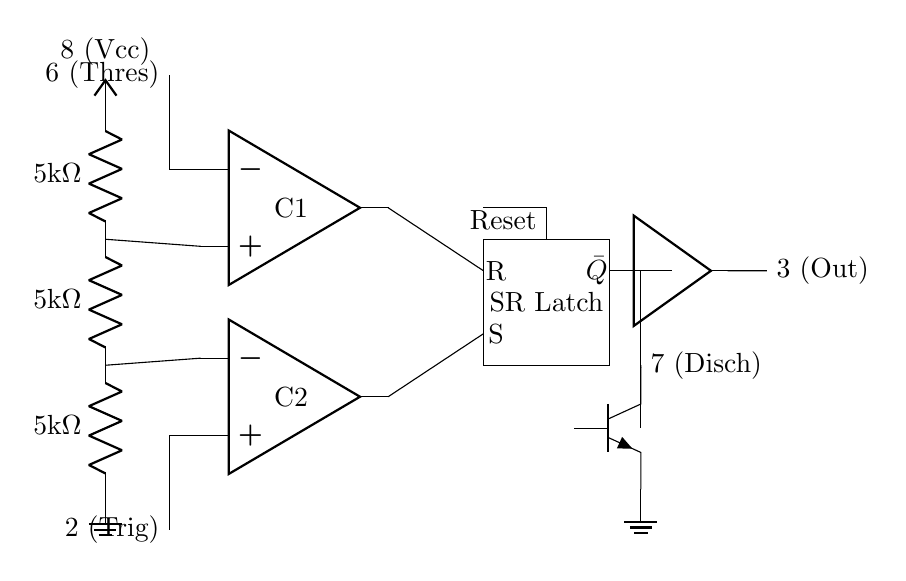
\begin{tikzpicture}[scale=0.8]
    % Voltage Divider
    \draw (0,0) node[ground] {} to[R, l=5k\(\Omega\)] (0,2) to[R, l=5k\(\Omega\)] (0,4) to[R, l=5k\(\Omega\)] (0,6) node[vcc] {8 (Vcc)};
    
    % Comparators
    \draw (3,1.5) node[op amp] (C2) {C2}; % Trigger
    \draw (3,4.5) node[op amp] (C1) {C1}; % Threshold
    
    % Connections to Comparators
    \draw (C2.+) -- ++(-0.5,0) -- ++(0,-1.5) node[left] {2 (Trig)};
    \draw (0,2) -- (C2.-);
    \draw (C1.-) -- ++(-0.5,0) -- ++(0,1.5) node[left] {6 (Thres)};
    \draw (0,4) -- (C1.+);
    
    % Flip Flop (SR Latch)
    \draw (6,2) rectangle (8,4);
    \node at (7,3) {SR Latch};
    \node at (6.2, 3.5) {R};
    \node at (6.2, 2.5) {S};
    \node at (7.8, 3.5) {\(\bar{Q}\)};
    
    % Connections to FF
    \draw (C1.out) -- (6, 3.5); % R
    \draw (C2.out) -- (6, 2.5); % S
    \draw (6, 4.5) -- (7, 4.5) -- (7, 4) node[above left] {Reset}; 
    
    % Output Stage
    \draw (8, 3.5) -- (9, 3.5) node[buffer] (buf) {}; % Inverting buffer usually
    \draw (buf.out) -- (10.5, 3.5) node[right] {3 (Out)};
    
    % Discharge Stage
    \draw (8, 3.5) -- (8.5, 3.5) -- (8.5, 1) node[npn] (T) {};
    \draw (T.E) node[ground] {};
    \draw (T.C) -- (8.5, 2) node[right] {7 (Disch)};
    
\end{tikzpicture}
\caption{IC 555 Functional Block Diagram}
\end{figure}

\paragraph{Mnemonic:}
\emph{3 Resistors (5k), 2 Comparators, 1 Flip-Flop, 1 Transistor (Discharge).}


% ========================================
% QUESTION 5(c) OR: Astable Multivibrator (7 marks)
% Demonstrates: Circuit, Operation
% ========================================

\subsection{Question 5(c) OR [7 marks]}
\textbf{Draw and explain Astable Multivibrator using IC 555.}

\subsubsection{Solution}
An Astable Multivibrator has no stable state. It switches continuously between High and Low states, producing a square wave output (Free-running Oscillator).

\paragraph{Circuit Diagram:}
\begin{figure}[H]
\centering
\begin{circuitikz}[scale=1]
    \draw (0,0) node[dipchip, num pins=8, hide numbers, no topmark, external pins width=0](C){IC 555};
    
    % Pin Connections
    \draw (C.pin 1) -- ++(-0.5,0) node[ground]{} node[left, pos=1]{1 (GND)};
    \draw (C.pin 8) -- ++(0,1) node[vcc]{Vcc} node[right, pos=0.1]{8};
    \draw (C.pin 4) -- ++(0,0.5) -- (C.pin 8); % Reset to Vcc
    
    % Timing RA, RB, C
    \draw (C.pin 8) ++ (2,1.5) node[vcc]{Vcc} to[R, l=\(R_A\)] ++(0,-1.5) coordinate (node7) -- (C.pin 7);
    \draw (node7) to[R, l=\(R_B\)] ++(0,-1.5) coordinate (node62);
    \draw (node62) to[C, l=\(C\)] ++(0,-1.5) node[ground]{};
    
    % Connect 6 and 2 to capacitor
    \draw (node62) -- (C.pin 6);
    \draw (node62) -- ++(0.5,0) -- ++(0, -2.5) -- ++(-4,0) |- (C.pin 2);
    
    % Control Voltage
    \draw (C.pin 5) to[C, l=0.01\(\mu\)F] ++(0,-1) node[ground]{};
    
    % Output
    \draw (C.pin 3) -- ++(1,0) node[right]{Output (Square Wave)};
    
    \node at (C.bpin 1) [left, font=\tiny] {GND};
    \node at (C.bpin 2) [left, font=\tiny] {TRIG};
    \node at (C.bpin 3) [right, font=\tiny] {OUT};
    \node at (C.bpin 4) [left, font=\tiny] {RST};
    \node at (C.bpin 5) [right, font=\tiny] {CV};
    \node at (C.bpin 6) [right, font=\tiny] {THR};
    \node at (C.bpin 7) [right, font=\tiny] {DIS};
    \node at (C.bpin 8) [left, font=\tiny] {VCC};
\end{circuitikz}
\caption{Astable Multivibrator Circuit}
\end{figure}

\paragraph{Operation:}
\begin{enumerate}
    \item \textbf{Charging:} Capacitor C charges through \(R_A\) and \(R_B\) towards \(V_{cc}\). The output is High.
    \item \textbf{Threshold Reached:} When capacitor voltage reaches \(2/3 V_{cc}\), pin 6 resets the flip-flop. The output goes Low.
    \item \textbf{Discharging:} Pin 7 opens to ground. The capacitor discharges through \(R_B\) into pin 7.
    \item \textbf{Trigger Reached:} When capacitor voltage drops to \(1/3 V_{cc}\), pin 2 sets the flip-flop. The output goes High, and the cycle repeats.
\end{enumerate}

\paragraph{Frequency Formula:}
\[ f = \frac{1.44}{(R_A + 2R_B)C} \]
\[ \text{High Time } T_{on} = 0.693 (R_A + R_B) C \]
\[ \text{Low Time } T_{off} = 0.693 (R_B) C \]

\paragraph{Mnemonic:}
\emph{\(R_A\) and \(R_B\) charge. Only \(R_B\) discharges. Toggle between 1/3 and 2/3 Vcc.}

\end{document}
